\section{PID-control}


As has been seen in previous sections, it can be difficult to model the system. If it is possible to find a method that may control the plant, without having to rely on overly complex models or unreliable estimates, that would be desirable. Fortunately, normal cascaded PID-controllers can very often do an excellent job without an exact model. PID-controllers also often have the advantage of being robust against modelling errors. Unfortunately, tuning the three parameters in a PID-controller is known for being a difficult task, depending on the type of process. As a result, several different methods have been developed for tuning PID-controllers. This section will explain how to tune a PI or PID-controller by using Skogstad's Internal Mode Control (SIMC). 


\subsection{Skogstad's Internal Mode Control}

SIMC is a set of rules for tuning PID-controllers that were originally used for teaching-purposes, but who have proven to work very well in practice. The method is based, quite simply on exciting the system form a stationary state with a step-response. A step-response is often more well-behaved on most systems, and usually gives a response that is more in line with that of an actual linear system. The SIMC are the tuning rules for how to tune the constants of a PID-controller if a simple approximation of the model is already known. As a result, there are two parts of SIMC-tuning. The system approximation and the actual tuning. Because parts of the system are also affected by a rather large non-minimum phase response, it will also be necessary to expand upon the normal system approximation to handle the large transients. 





\subsection{Simplifying plant models}

Skogstad's method normally relies on some transfer function model of the system to tune the system. If $\tau$ represents the lag in the system and $e^{\theta_0 s}$ represents the delay and $k$ the plant gain, then Skogstad's method is based on a SISO (Single Input Single Output)  system that can be described as: 

\begin{align}
    y = k \cdot \frac{\prod_{i=1}^{n}  \left(  - T^{inv}_i s + 1\right)}{\prod_{j=1}^{n} \left( \tau_{j,0} s +1  \right)} e^{-\theta_{0} s}
\end{align}
Where $\tau_i \geq \tau_{i+1} \geq 0$ and $T^{inv}_i \geq T^{inv}_{i+1} \ge 0$ (Positive roots in the numerators are explained in subsection \ref{sec:positive_numerator_time_constants}). Since Skogstad's method only revolves around a PID-controller, only the most dominant terms are taken into consideration. Any factor after the second one will instead be approxomated by a the Taylor-approxomation of a time-delay and added to the already existing time-delay. 

\begin{align}
    e^{\tau_j s} &= 1 + \tau_j s + \dots \tau_j^i s^i + \dots &\approx 1 + \tau_j s \\
    e^{-\tau_j s} &= \frac{1}{e^{\tau_j s}} &\approx \frac{1}{\tau_j s +1}
\end{align}

\noindent
Depending on the properties of the plant, it is possible to perform different simplifications. If the lag $\tau_1$ dominates the process (usually $\tau_1 > 8\theta$), then the estimation $\frac{k}{\tau_1 s +1} \approx \frac{k'}{s}$ can be used. This can also alow you to end the experiment early instead of waiting for convergence. 
A discretely sampled with a sampling time $h$, can be simplified into a continuous system with an additional time-delay $\frac{h}{2}$  if the time-delay is not too dominant. Additionally, the largest neglected pole can be evenly distributed between the smallest lag that is being used and the time-delay.

\noindent 
All these rules can be summarized into the much simpler rules, described in equations \ref{eq:SIMC_approx_2nd_order} and \ref{eq:SIMC_approx_1st_order}. The tuning rules are lifted dirextly from equations (10) and (11) in \cite{SIMC_source}. 

\colorbox{gray}{\begin{minipage}{\textwidth}
    Second order approxomation :
\begin{align}
    \label{eq:SIMC_approx_2nd_order}
    \tau_1 = \tau_{1,0};&\tau_2 = \tau_{2,0} + \frac{ \tau_{3,0}}{2}; \theta = \theta_0 + \frac{\tau_{3,0}}{2} + \sum_{i \ge 4} \tau_{i,0} + \sum_j T^{inv}_{j0} \ \frac{h}{2}
\end{align}

First order approxomation: 
\begin{align}
    \label{eq:SIMC_approx_1st_order}
    \tau_1 = \tau_{1,0} + \frac{\tau_{2,0}}{2} ; \theta = \theta_0 + \frac{\tau_{2,0}}{2}  \sum_{i \ge 3} \tau_{i,0} + \sum_j T^{inv}_{j0} \ \frac{h}{2}
\end{align}
\end{minipage}}

\subsubsection{Positive time-constants in the numerator}
\label{sec:positive_numerator_time_constants}
In \cite{SIMC_source} positive roots in the numerator $\left( T_0 s +1 \right)$ are handled by allowing the term in the numerator to cancel one in the denominator (The closest, larger one). The delay $ \theta$ is the final delay after all cancellations have been made. Because of this, the cancellations have to be made iteratively with the new delays.

\begin{align}
    \frac{T_0 s +1}{\tau_0 s +1} \approx 
    \begin{cases}
        \frac{T_0}{\tau_0} & \text{if } T_0 \ge \tau_0 \ge \theta\\
        \frac{T_0}{\theta} & \text{if } T_0 \ge \theta \ge \tau_0\\
        1 & \text{if } \theta \ge T_0 \ge \tau_0\\
        \frac{T_0}{\tau_0} & \text{if } \tau_0 \ge T_0 \ge 5 \theta\\
        \frac{\left( \tilde{ \tau }_0 / \tau_0 \right)}{\left( \tilde{\tau}_0 - T_0  \right)s +1} & \text{if }  \tilde{\tau}_0 \delequal \text{min} \left( \tau_0, 5 \theta \right) \ge  T_0 
    \end{cases}
\end{align}
If there is no larger time-constant in the denominator, the closest smaller one is used instead. 

\subsection{PID-rules}
SIMC uses the IMC tuning rules for generating the PID-parameters after a first or second-order model has been found. A more complete derivation of the rules is found in \cite{SIMC_source}, but the short version is: 

\noindent
Usually, a desired response with time-constant $\tau_c$ is selected. $\tau_c$ is a tuning constant of the SIMC, that is the desired time-constant of the closed-loop system. 
\begin{align}
    \left(\frac{y}{y_{s}}\right)_{desired} = \frac{1}{\tau_c s +1} e^{\theta s}
\end{align}
 Let $g(s)$ be the transfer-function that describes the plant. An ideal controller $c^*(s)$ is choses such that if 
 \begin{align}
     g(s) = \frac{k}{\left( \tau_1 s+1 \right) \left( \tau_2 s +1 \right)} e^{\theta s}
 \end{align}
Then, the idealised controller can be writen as:
 \todo[inline]{I lef off correction here @@@}
 \begin{align}
    \frac{g(s) c^*(s)}{1 + g(s) c^*(s)} = \left(\frac{y}{y_{s}}\right)_{desired}
 \end{align}
\begin{align}
    c^*(s) = \frac{\left( \tau_1 s +1 \right)\left( \tau_2 s +1 \right)}{k} \frac{1}{\tau_c s+1 - e^{- \theta s}}
\end{align}
The Taylor-approxomation is used to get rid of the $e^{-\theta s} \approx 1 - \theta s$, such that the approxomated controller $c(s)$ becomes
\begin{align}
    \label{eq:delay_controller}
    c(s) = \frac{\left( \tau_1 s +1 \right)\left( \tau_2 s +1 \right)}{k} \frac{1}{\left( \tau_c + \theta \right)s}
\end{align}
becomes $ \left(\left( \tau_c + \theta \right)s\right)$. However, if the lag is the most dominant part of the process, this kind of tuning will result in a very slow setling-time.  This is solved by approximating the system as a pure integrating process with no $ \frac{k}{\tau_1 s +1 } e^{- \theta s} \approx \frac{k}{\tau_1 s} = \frac{k'}{s}$. Afterwards, $c(s)$ can be set as a PI-controller with gains that cause the closed loop to have a damping factor $\xi$ of 1
\begin{align}
    \label{eq:second_order_plant_feedback}
    \frac{g(s)c(s)}{1 + g(s)c(s)} = \frac{ \frac{k'}{s} K_c \left(1+ \frac{1}{\tau_I s}\right)}{1 + \frac{k'}{s} K_c \left(1+ \frac{1}{\tau_I s}\right)}
\end{align}
Sorting out the terms gives 
\begin{align}
    \frac{\tau_I s + 1}{\frac{\tau_I }{k' K_c}s^2 + \tau_I s + 1}
\end{align}

\noindent
A system on standard second order form is written as $\tau_0^2 s^2 + 2\tau_0 \xi s +1$. If $\xi =1$, any system with denominator on that form is critically damped. So, in the case of equation \ref{eq:second_order_plant_feedback}

\begin{align}
    \tau_0 = \sqrt{\frac{\tau_I}{k' K_c}}\\
    \xi = \frac{1}{2} \sqrt{k' K_c \tau_I}
\end{align}

\noindent
So if $K_c$  is chosen as in equation \ref{eq:delay_controller} to be $ \frac{1}{k} \frac{\tau_1}{\tau_c + \theta} $, then $\tau_I = 4\left(\tau_c + \theta \right)$. Both these tuning rules can be combined into one very simple one. 

\colorbox{gray}{\begin{minipage}{\textwidth}
\begin{align}
    \label{eq:SIMC_simple_tuning_rule}
    K_c     &= \frac{1}{k} \frac{\tau_1}{\tau_c + \theta}\\
    \tau_I  &= \text{min} \left\{ \tau_1, 4 \left( \tau_c + \theta \right)\right\}\\
    \tau_D  &= \tau_2
\end{align}
\end{minipage}}

\noindent
If a PI-controller is needed, a simpler model is used instead, such that $\tau_2 =0$. \cite{SIMC_source} mentions that $\tau_c \in [\theta , \infty)$ can be chosen freely, but that it is a tradeoff between speed and robustness (as well as smaller variations in inputs). The paper highlights that $\tau_c = \theta$ is a good tradeoff between speed and robustness. 


   



\subsection{PID-tuning by using bode-plots}


Although Skogstad's method can be very useful, it might sometimes struggle with systems where the poles or zeros are complex, since those cases are not defined in the original method. There are proposed methods for handling such cases, but it is also possible to simply tune a stable system by observing the phase-response of a stable system and choosing $K_{c}$ and $T_{I}$ such that a sufficient phase and gain margin can be achieved. If the system is stable and the controller is a simple PI-controller, then it is also possible to find a set of rules that can automate the tuning-process, so that it is robust against time-delays and modelling errors.

\subsubsection{A quick reintroduction to bode-plots (Nyquist's criteria of stability)}

Let the transfer-function of the plant be $h_p(s)$, and the transfer-function of the controller be $h_c(s)$. Let $h_0(s) = h_p(s) h_c(s)$ An instability in the system is caused if the transfer-function of the closed loop 

\begin{align}
    M(s) = \frac{h_0(s)}{1 + h_0(s)}
\end{align}
has a pole in the left half-plane. $1+ h_0(s)$ can be divided into a numerator and denominator, and the resulting closed-loop will have a set of poles and zeros 
\begin{align}
    1+ h_0(s) = 1 + \frac{n_0(s)}{d_0(s)} = \frac{d_0(s) + n_0(s)}{d_0(s)} = \frac{(s -\lambda_1) \dots ( s -\lambda_n)}{(s-\rho_1)\dots (s-\rho_n)}
\end{align}
If one performs integration of s along the imaginary axis, and then along a circle with an infinitely large radius in the right half-plane, only poles and zeros in the right half-plane will give a net contribution to the phase, as described in \cite{Regtek_boken}. This can be seen in figure \ref{fig:Nyquist_criteria}. All zeros $\lambda$ will give a net negative contribution to the angle, while all poles $\rho$ will give a positive contribution. 



\begin{figure}[h!]
    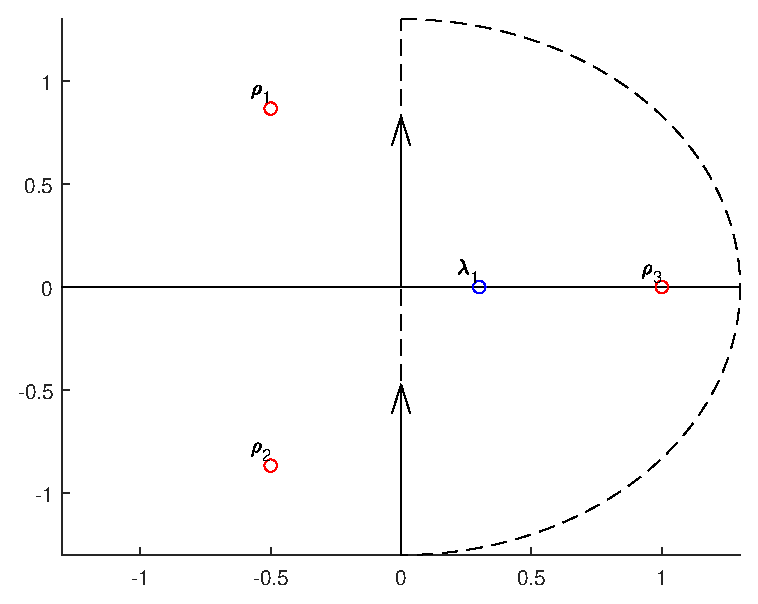
\includegraphics[width=\textwidth]{img/Fig_dump/Nyquist_criterion.eps}
    \caption{Poles $\rho$ and zeros $\lambda$ of a transfer-function. The existence of $\rho_3$ makes it unstable}
    \label{fig:Nyquist_criteria}
  \end{figure}

\noindent
$\Delta \angle (1 + h_0(s))$ is the total angular change when integrating along the half-circle. $N_p$ and $N_n$  are the total number of poles in the right half-plane in the open and closed system respectively. The resulting relation is 

\begin{align}
    \Delta \angle (1 + h_0(s)) = - 2\pi \left( N_n- N_p \right)
\end{align}
So, Nyquist's stability criteria uses the total phase-contribution of $1+h_0(s)$, and the number of unstable poles in the open-loop system to determine the number of unstable poles in the closed-loop 

\begin{align}
    N_n = N_p - \frac{\Delta \angle (1 + h_0(s))}{2\pi} 
    \label{eq:nequist_stability_criteria}
\end{align}
\noindent
To analyze if an open loop system will be stable when the loop is closed, a bode-plot, like in figure \ref{fig:generic_bode_plot} is normally used. A bode-plot consists of one plot of the amplitude of the open-loop, and the phase of the open-loop system. Both of them are plotted against an angular velocity, $\omega$.
\todo[inline]{Get figures that are cropped better }
\begin{figure}[ht]
    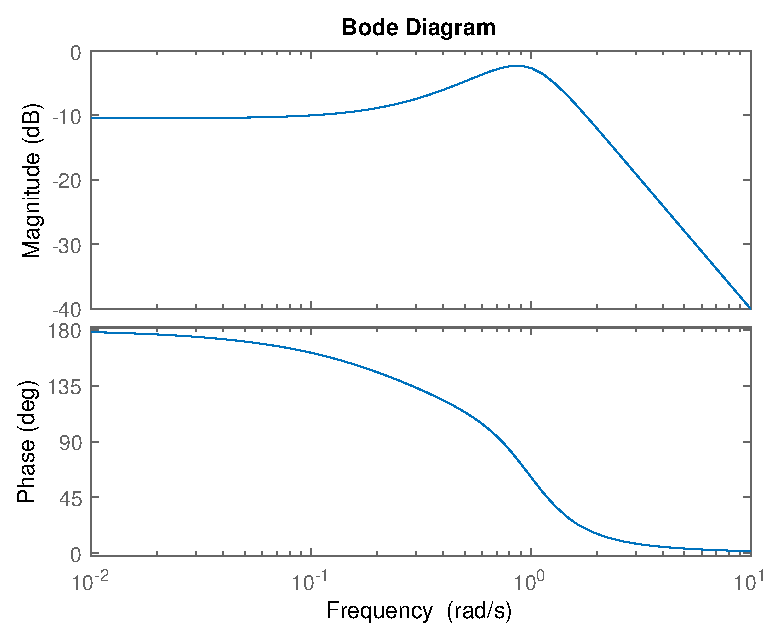
\includegraphics[width=\textwidth]{img/Fig_dump/Generic_bode_plot.eps}
    \caption{A generic bode-plot of $\frac{s-0.3}{s^2 + s + 1}$}.
    \label{fig:generic_bode_plot}
\end{figure}


\noindent
A bode-plot makes it very clear a stable system will be stable in a closed-loop as well. If the amplitude of $h_0(s)$ is greater than 1 (0 dB) when the phase is modulo 360 is -180 degrees, then the system is unstable. 



\subsection{Gain and phase margins of stable systems}


The plant that is being controlled is known to be stable, so the only condition that has to be satisfied is that the amplitude of the system is less than 0dB whenever the phase of the system crosses $-180^o$. It is never possible to know exactly how one might model the system incorrectly, but bode plots allow saying something about the robustness against time-delays and against unknown gains affecting the system. If a system has robustness in both of these regards, then it should also have some robustness to in regards to the modelling errors with regards to the system dynamics as well. 


\noindent
Since time-delays are written as $e^{\theta j \omega}$, they only contribute with an addition to the phase in the bode-plot. This means that a good phase-margin will give robustness against time-delays. Usually, it is said that a phase margin of $60^o$ and a gain margin of 20dB is a good balance between performance and robustness. 



\noindent

\subsubsection{Choosing a good controller}

One way to say something about a controller is by using the control ratio $N(s) = \frac{1}{1 + h_0(s)}$ and the following ratio $M(s) = \frac{h_0(s)}{1 + h_0(s)}$. $M$ tells how the system will track changing references of a given frequency, as a result, it will also say how much the system reacts to measurement noise. Meanwhile, N says how well noise or disturbance will be suppressed. When working with a system that is subject to both noise and process disturbances, both $N(s)$ and $M(s)$ are necessary. Ideally, $N(s)$ has such a shape that all disturbances become 0 while ignoring any noise. This is impossible, but it gives a hint as to how the controller and filters would be chosen. If it is known that some noise has a very specific frequency, then band-stop filters or notch-filters can be added to the controller as well. 
\begin{figure}[!ht]
    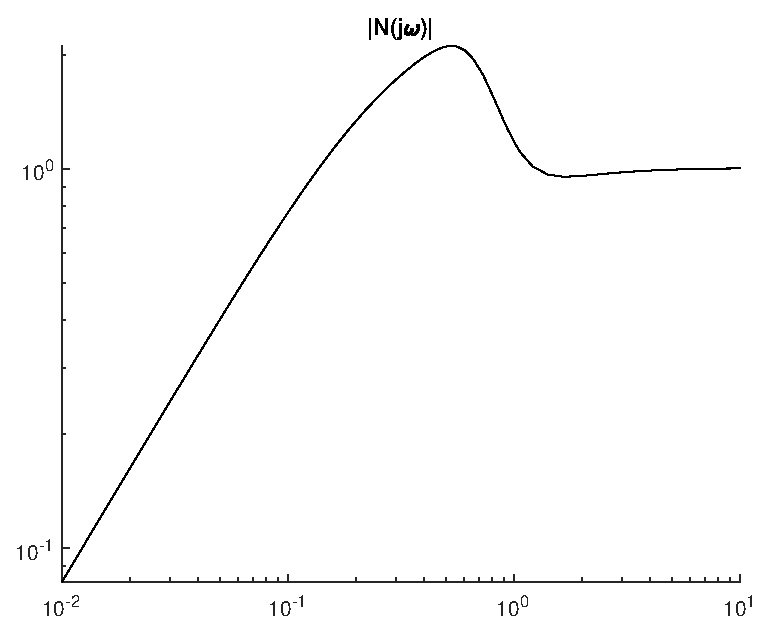
\includegraphics[width=\textwidth]{img/Fig_dump/Generic_N_plot.eps}
    \caption{N for a poorly controlled process}
    \label{fig:N_plot}
\end{figure}


\noindent
In figure \ref{fig:N_plot}, a plot of $N(j\omega)$ is given for some arbitrarily chosen controller. As can be seen in the plot, it does suppress disturbances at low frequencies. Additionally, it can be seen that for high frequences, the disturbances are simply let through. However, a rather large peak at around $0.3  \frac{rad}{s}$ can be seen as well. This peak around where the crossover-frequency, which means that $h_0(j\omega)$ almost entirely negative. As long as the phase of $h_0(j \omega)$ crosses $-180^o$, there is always a point where the amplitude of $N(j \omega) > 1$. The way to control the size of this peak is by making sure the amplitude of $h_0(s)$ is sufficiently small around $-180^o$, since if it were to be close to 1, then the system would amplify any noise or disturbance of that frequency by an almost absurd amount.


\noindent
There are two possible measures that can be taken to supress the resonance around the unwanted frequencies. The first is to simply increase the gain margin. If the amplitude of $h_o(j \omega)$ is small at $\angle h_o(j \omega) \approx -180$, then the fraction $\frac{1}{1 + h_0(j \omega)}$ does not grow as large. A phase margin of $20dB$ will ensure that the resonant amplitude will be less than $\frac{1}{1 - \frac{1}{10}} \approx 1.11$. 

\noindent
The second option is to use the D-part of the controller to "lift" the phase of the combined controller and plant. Normally, most plants attenuate high-frequency signals more than low-frequency ones, so by keeping the phase above $-180^o$ for longer, $|h_0(s)|$ can be made to be smaller at the new crossover frequency. Simply adding a differentiating term can sometimes lead to other problems, since it makes the system react more to high-frequency noise. The solution is to add a low-pass filter to the controller as well. An additional advantage of using a low-pass filter is that a differentiation term will usually require some numerical differentiation, that might be ill-behaved. A differentiation term in series with a low-pass filter gives a variation of a high-pass filter, which is a proper transfer function\footnote{Proper transfer function: The order of the denominator (Highest  degree of s) is greater or equal to the order of the numerator}, that can be written as a causal system and discretized in a more well-defined manner. 


\noindent

The need for low-pass filters can be shown in figure \ref{fig:M_plot}. Even if the plot for $N(s)$ looked good, $M(s)$ shows that high-frequency noise are not sufficiently attenuated, making it susceptible to noise, which is very often present in the form of electrical noise. 

\begin{figure}[!ht]
    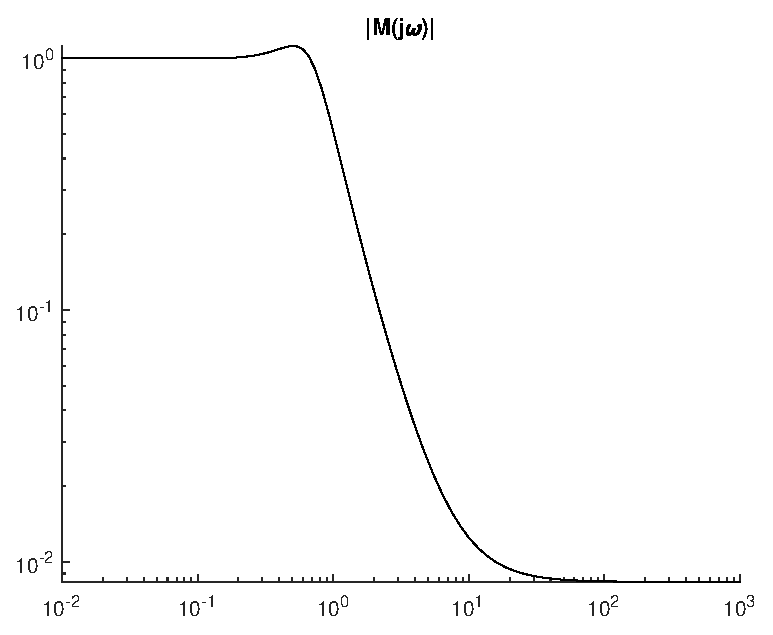
\includegraphics[width=\textwidth]{img/Fig_dump/Generic_M_plot.eps}
    \caption{M for a poorly controlled process}
    \label{fig:M_plot}
\end{figure}


\todo[inline]{I left off here}


% This can potentially be very bad if the system is subjected to the noise around those frequencies. The amplification of the noise is because of $h_0(j\omega)$ being almost purely negative and real at those frequencies. Preferably, $K_c$ should be chosen, such that $h_0(s)$ has a small amplitude when the phase is close to $-180$. This can be done by using a gain-margin that is sufficiently large. 



% Although we do not know the frequencies that make up the noise, it seems reasonable that there are patterns that happens hourly or daily (A change in quality, depending on the day, or if new waste is added roughly every hour). If a controller has terms that resonate around that frequency, then that is a bad choice for a controller. The good part about the controller is that $N(j\omega) \approx 1$ for all frequencies above $10^{-1}$ since the worst noise is most likely the disturbances that come from from the measurements in some form. 



\todo[inline]{Find the real names of M and N}






